\documentclass[]{article}
\usepackage{amsmath}
\usepackage[utf8x]{inputenc}
\usepackage{color}
\usepackage{tikz}
\usepackage{graphicx}
\usepackage{subfig}
\usepackage{tikz-cd}
\usetikzlibrary{decorations.pathmorphing}

\usepackage[ukrainian]{babel}
\author{Березюк~Іван}
\graphicspath{ {img/} }

\title{ Звіт з науково-виробничої практики \\ 
		студента 2-го курсу магістратури \\
		кафедра Ядерної фізики\\
		Науковий керівник: Massimiliano Ferro-Luzzi\\ 
		}

\begin{document}

	\maketitle
	\newpage
	\section{ План роботи}
	\begin{itemize}
		\item Розраховано калібувальну криву, для реконструкції позиції треків відносно центру дрейфової трубку для MIP(minimum ionising particles - мінімум іонізуючих частнок) на прикладі мюонів з енергією 1 ГеВ (знаходиться обернена залежність $r(t)$ від розподілу "час дрейфу $t$ як функція положення $r$ треку відносно проводу").\par
		\item Провів симуляцію 50 тисяч треків через дрейфову трубку випадковим чином з рівномірним розподілом. По аналізу сигналу кожного треку було визначено час дрейфу електронів і реконструйовано розподіл позиціонування кожного треку. По отриманим даним було побувано діаграми густини розподілу відхилення $r_{real} - r_{reconstructed}$ як функція від $r_{real}$.
	
		\item Після врахування всіх ефектів, що можуть впливати на вхідний сигнал необхідно реєструвати час приходу сигналу подібно дискримінатору імпульсів і використати даний алгоритм в для даних Garfield для побудови калібрувальної кривої і решти розрахункуів.
	\end{itemize}

	\newpage
	\section{Теоретичний вступ}
		Рідкісні розпади $ K \rightarrow \pi\nu \overline{\nu} $ є чудовим знаряддям вивчення фізики ароматів із-за своєї чистої природи. Дякуючи сильному GIM механізму, ці розпади є домінуючими в короткодистанційній динаміці. Окрім того, коротко-дистанційна амплітуда регулюється лише єдиним напівлептонним оператором, чий адронний матричний елемент вимірюєтсья експриментально з аналізу данниих від напівлептонних розпадів. Фактично це означає, що найбільші теоретичні невизначеності в цьому випадку можуть бути перевірені чисто експериментально.
		
		Так як пара нейтрино-антинейтрино є частинками які фактично неможливо зареєструвати а тим більше визначити їх треки, то козпад $K^+$ визначається лише по треку дочірньої $\pi+$ частинки. Тож для для реконструкції вершини розпаду необхідно знати часові та просторові характеристики треків від $K^+$ ,$\pi^+$ та всіх інших частинок, суміжних з даною реакцією та іншими фоновими процесами з точністю необхідною для вияснення причинно-наслідкового зв’язку.
		
		Конкуруючими процесами до розпаду 
		$ K^+ \rightarrow \pi^+\nu \overline{\nu} $ є 
		$ K^+ \rightarrow \pi^+\pi^0 $, 
		$ K^+ \rightarrow \mu^+ \nu $ та 
		$ K^+ \rightarrow \pi^+ \pi^+ \pi^- $ розпади.
		
		\section{Формулювання задачі}
		Для визначення треків заряджених $\pi$ та $\mu$ частинок в експерименті SHiP пропонується використовувати детекторну систему на базі дрейфових трубок.
		
		Для цієї трекової детекторної системи ствиться декілька вимог:
		\begin{itemize}
		\item забезпечити необхідну точність визначення треку на рівні $100 \mu m$
		\item ефективна товщина системи не повинна перевищувати $2\%$ радіаційної довжини
		\item точність визначення імпульсу частинки має бути на рівні $0.5\%$ обо ж нижче.
\end{itemize}
		Виконання всіх цих вимог дозволить отримати роздільну здатність по масі на рівні $10^{-3}~GeV^2 / c^4$, що має бути достатньо для поставленої задачі.
		\section{Трековий частина детектора}
		Трековий детектор має складатися з двох частин - каонного та піонного. По суті це тонкі детектори розташовані перперндикулярно до напряму пучка, в області розташування яких діє сильне штучне магнітне поле. Каонний спектроментр являє собою три послідовно розташовані твердотільні піксельні детектори.
		
		Піонний спектрометр в свою чергу складається з шарів дрейфових трубок розташованих в середині вакуумного танкеру. Вибір STRAW трекера у вакуумі був зроблений з міркувань зменшення інтенсивності багаторазового розсіяння частинок пучка на конструкційних матеріалах.
		
		STRAW трекер є предметом дослідження дарої роботи. Визначення його роздільної спроможності та пошук кращих дизайнерських рішень з метою поліпшення його просторово роздільної спроможності в межах даного експерименту.
		 
		\section{Параметри STRAW детектору}
		Параметри STRAW трекеру такі ж як і у випадку експерименту NA62 з єдиною головною відмінністю -- вони стали довшими($5m$ проти $2.1m$ у випадку NA62). В наступній таблиці описані параметри дрейфових трубок.
		
	\begin{tabular}{|l|l|p{8cm}|}
		\hline
		Величина & Значення\\
		\hline
		радіус дроту & $30\mu m$\\
		\hline
		матеріал дроту & gold-plated Thungsten\\
		\hline
		довжина дроту & $5m$ \\
		\hline
		потенціал дроту & $1750 V$ \\
		\hline
		потенціал стінок трубки & $0 V$ \\
		\hline
		Внутрішній радіус трубки & $9.8~mm$ \\
		\hline
		Густина дроту & $19.3 ~g/cm^3$ \\
		\hline
		сила натягу дроту & $\sim 90~g$ \\
		\hline
		склад газової суміші в трубці & $Ar70\% ~CO_2 30\%$ \\
		\hline
	\end{tabular}
	
	Дріт всередині трубки має масу і під дією гравітаційного та електричного поля всередині трубки значно "провисає" (Рис. \ref{fig:sagProfile})
	
	\begin{figure}[h]
	\centering
	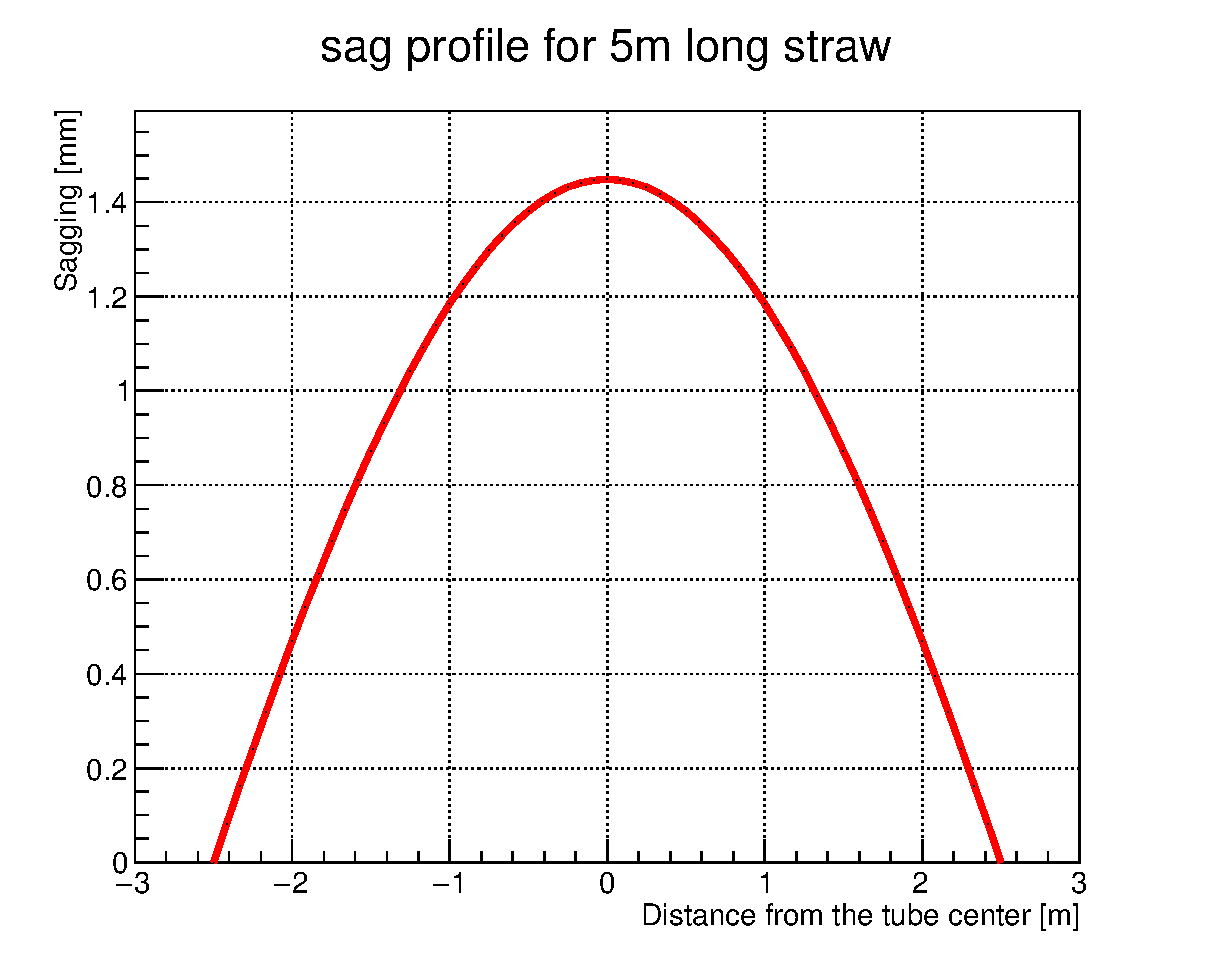
\includegraphics[width=0.5\textwidth]{sagProfileFit.eps}
	\caption{Профіль провисання проводу в дрейфовій трубці довжиною 5 метрів під дією електричного та гравітаційного полів розрaхований у програмному пакеті Garfield }
	\label{fig:sagProfile}
	\end{figure}	
	
	Це є чи на найбільшою проблемою при роботі з дрейфовими трубками, так як в залежності від зміщення трубки від центрального положення змінюється і час дрейфу. Це начно ускладнює процес реконструкції треків, і вимагає додаткових зусиль. При чому потрібно зважати на той обсяг інформації який ми можемо витягти з дрейової трубки в робочому стані. Адже не всі методи зостосовні до калібровки трубки в лабораторних умовах можуть бути виконані на практиці при в зібраному детекторі.
	
	Під дією сильного електричного поля дріт(анод $V_{wire}\cong1750 V$) притягується до стінок трубки (катод $V_{tube}=0V$) і так зване провисання досягає значних розмірів $\sim1.5mm$ при радіусі трубки всього $4.9 mm$. 

	Одним із головних припущень в даній задачі є вибір конфігурації трубок. Припустимо, що трубка є відносно ідеальна: не прогинається під дією гравітації та без викривлень в результаті дефектів при виробництві чи процесі встановленні на робоче місце, або ж якихось інших факторів). В умовах відсутності гравітаційного поля напрям провисання дроту передбачити неможливо - це повністю залежить від дефектів трубки при збірці та позиціонуванні дроту при фіксації на торцях.
	
	Проте в горизонтальному положенні трубок гравітаційного поля може бути достатньо щоб задати напрям провисання трубок строго вниз по напрямку гравітаційного поля $\vec{g}$. Таким чином неоднозначність конфігурації трубки пропадає.
	\begin{figure}[h]
		\centering
		\subfloat[Дріт без зміщення]{
			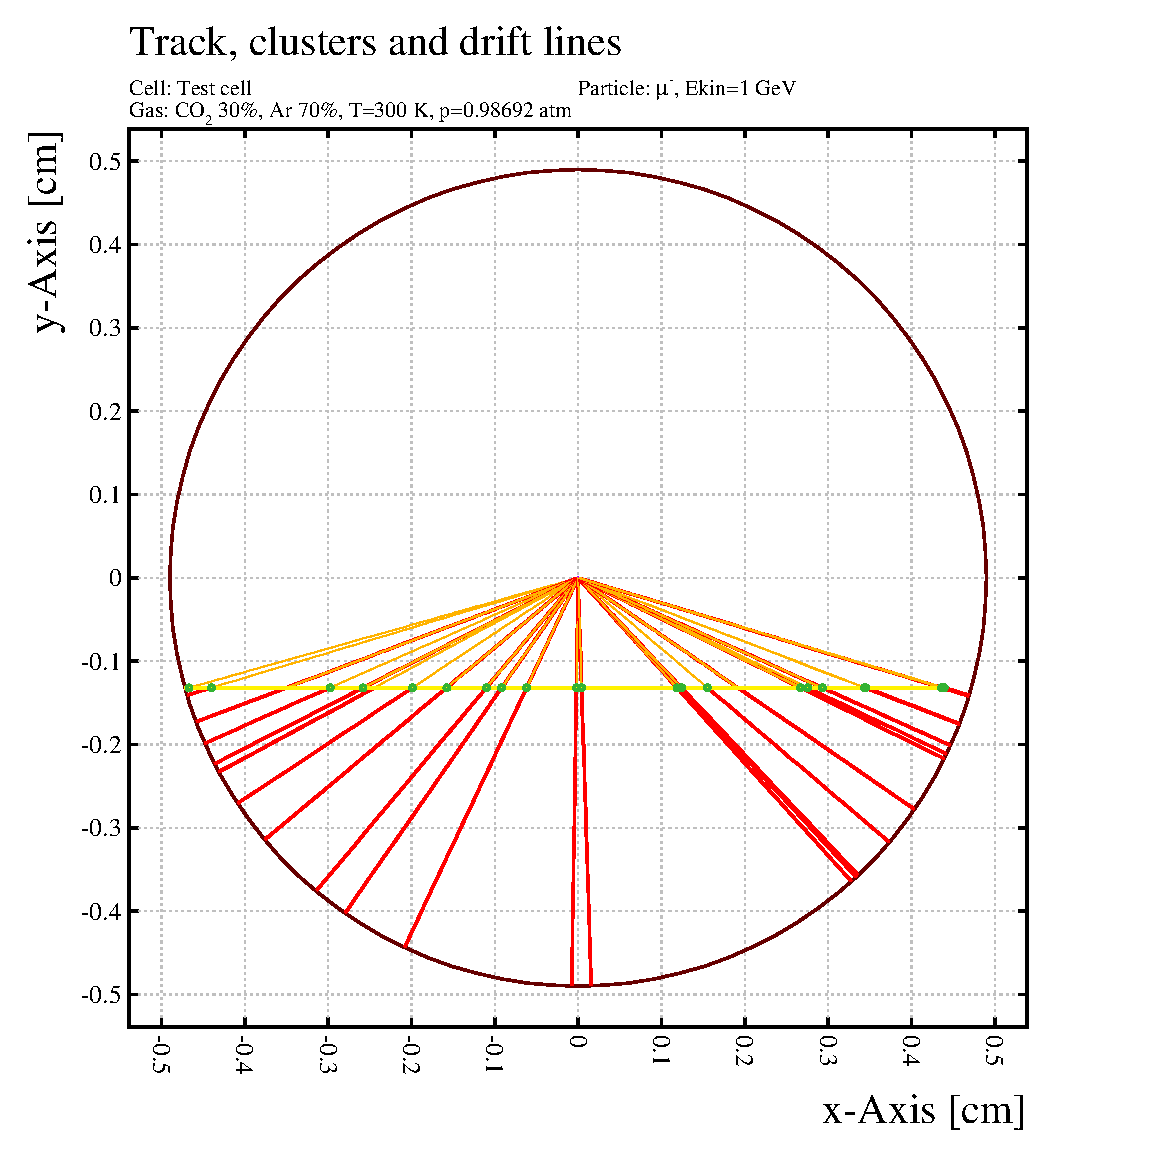
\includegraphics[width=0.45\textwidth]{tracksAndClusters00Sag.eps} 
			\label{fig:electron_ion_track} }%
		\qquad
		\subfloat[Зміщення $1.5 mm$]{
			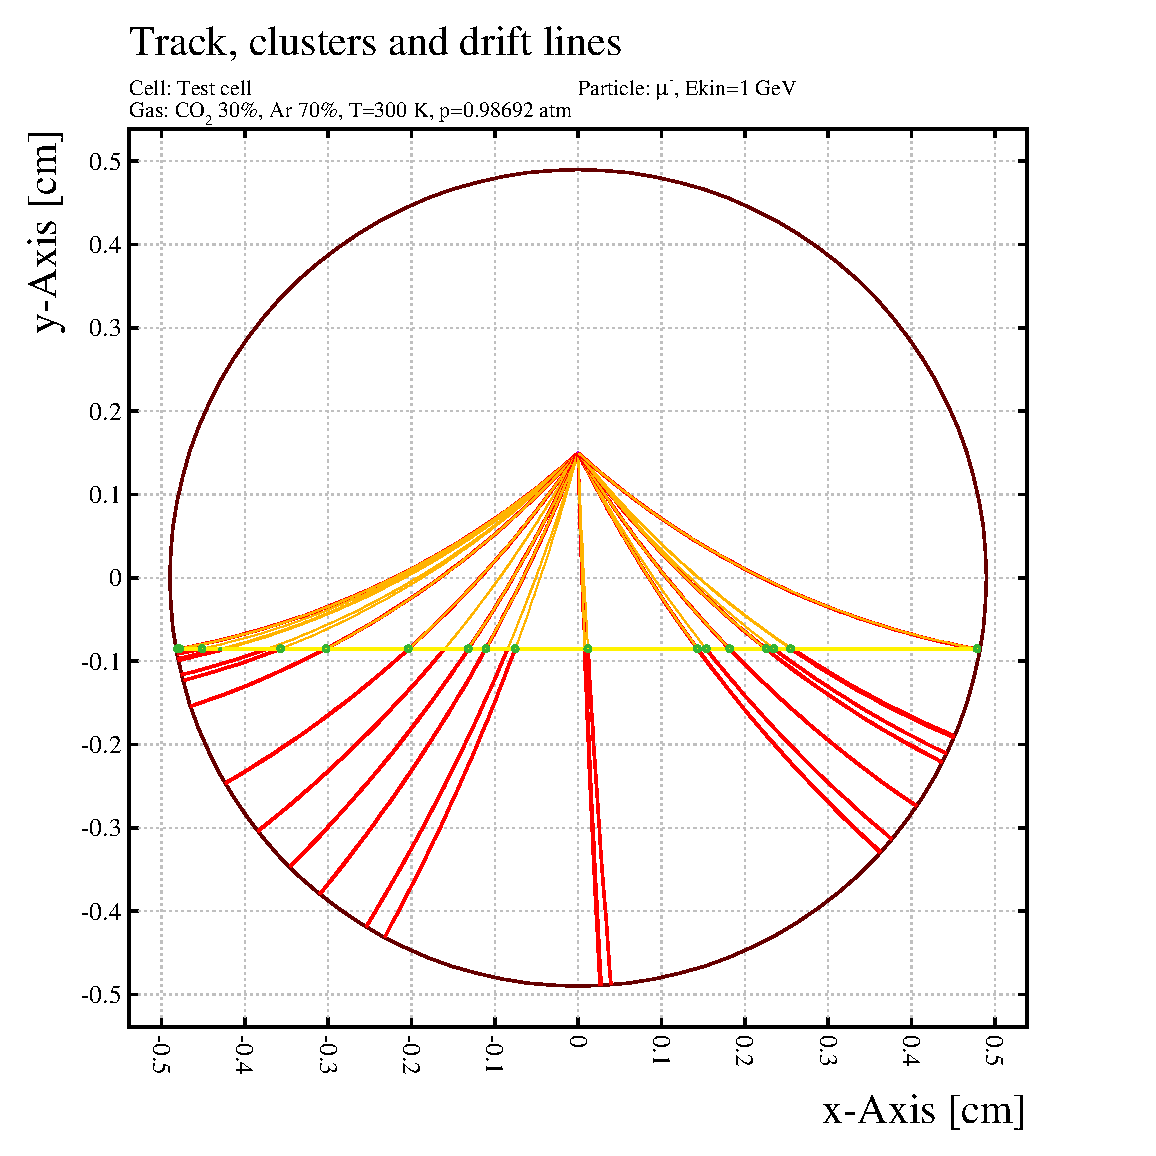
\includegraphics[width=0.45\textwidth]{tracksAndClusters15Sag.eps} 
			\label{fig:electron_ion_track_sag} }%
		\caption{ Приклад траекторії руху електронів та іонів в дрейфовій трубці в результаті проходження зарядженої частинки в горизонтальному напрямку(перпендикулярно до напрямку провисання трубки в площині поперечного перерізу дрейфової трубки}			
	\end{figure}
	
	\section{Сигнал}	
	Програмний пакет Garfield дає можливість просимулювати сигнал отримуваний від проходження частинки. 
	Figure \ref{fig:track_reconstruction} shows the schematic view of a particle passing the straw and producing ionization clusters along its path inside the straw. The number of produced ionization clusters directly affects the hit efficiency profile. \cite{kozlinskiy} Smaller ionization length increase hit efficiency, as more ionization clusters are produced.  After the ionization is produced the electrons drifts to the wire due to the electrical field between the wire and the straw. When the ionization cluster approaches the wire, the electrons ionize the gas due to the high electric field around the wire.  Subsequently a signal is induced on the wire and propagates to the readout electronics. The signal is registered if it passes a threshold value (Fig. \ref{fig:signal_example}). A variation of the signal height introduces a variation in the time when the
signal passes the threshold and is considered to be the main contribution to the STRAW tracker resolution. 

	In the track reconstruction software(GARFIELD \cite{garfield} an effective TR-relation is used. It only describes the relation between the drift time and the distance from the track to the wire, which differs from the distance to the ionization cluster. The shape of the TR-relation is defined by the drift velocity of the ionization cluster inside the straw. The electric field increases towards the wire, leading to a non linear TR-relation. Currently almost parabolic dependence is used, and easily can be fitted by \ref{eq:fit_tr} function.

	The drift time versus the unbiased distance distribution and the result of the fit are shown in Fig. \ref{fig:t_r_distr_00}. The noise hits under the main distribution, i.e. at earlier times, are due to primary or secondary particles ($\delta$-rays) passing the straw at a closer distance to the wire, consequently producing an earlier signal.
	
	За приклад в симуляціях в ролі частинки, що прошиває об’єм трубки будемо використовувати мюон $mu$ з енергією $1GeV$. Приклад треків від такої частинки видно на Рис. \ref{fig:electron_ion_track},\ref{fig:electron_ion_track_sag}. Зеленим кольором позначено точки локалізації кластерів іонізації визваної частинкою.
	
	До сигналу від треку також можна додати шум. Шум вибирався таким, щоб наближено дорівнював типовому. Вважаючи, що шум розподілений за пуассоном, RMS шуму вибирався на рівні максимального струму від 2000 електронів. На практиці шум дуже залежить від реалізації детектора, тому передчасно судити дуже важко. Однак ми не мали іншого вибору як цей.
	 
	На Рис. \ref{fig:signal_example} моментом часу Time=0 відповідає момент утворення первинних електрон-іонних пар від акту взаємодії мюона з атомами газую. Такий акт з великою точністю можна вважати миттєвим. Проте на експерименті такого фіксатора часу не буде. Тож відсутність передісторії сигналу погано вплине на точністю реконструкції, особливо якщо в схемі зчитування присутні інтегруючі ланки. В нашому випадку, це лише покращить кінцевий результат, так як все ще лишається імовірність того, що шум в колі все ще може перевищити порогове значення дискримінатора.
	
	\begin{figure}
	\centering
	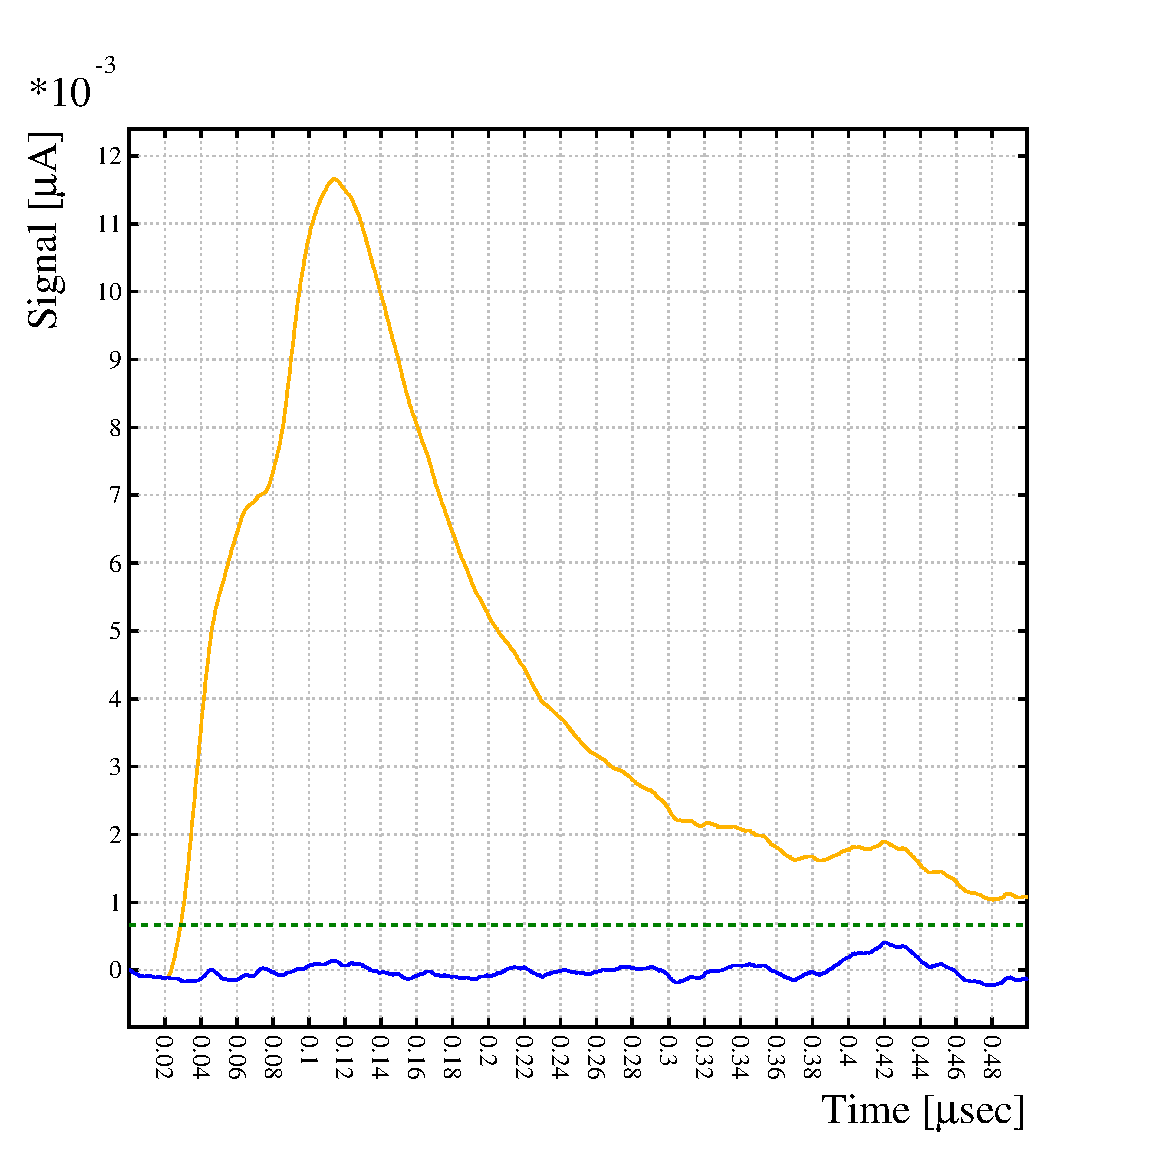
\includegraphics[width=0.7\textwidth]{signal_noise_threshold.eps}
	\caption{ Приблизний сигнал(напруга) на виході з формувача зчитувальної електроніки(жовта лінія). Складова шуму позначена синьою лінією. Зелена лінія відповідає напрузі 4 середніх квадратичних відхилень розподілу шуму. (Зазнач, що по осі Y величина суть напруга, проте домножена на сталий коефіцієнт, далекий від правди $\sim \frac{1}{Gain}$)}
	\label{fig:signal_example}
	\end{figure}
	
	\subsection{ STRAW efficiency}
		
	
	\section{Gain}
	Оцінка вихідного струму визначає front-end електроніку детектору. Коефіцієнт газового підсилення залежить від складових газової суміші, тиску, температури і поля в якому рухаються електрони/іони і розвиваються електрон-іонні лавини.
	
	Власне імплементація скрипту для розрахунку коефіцієнта підсилення вимагає від нас введення параметрів ефекту пеннінга \cite{} для розглядуваної газової суміші. Попри це механізм розрахунку коефіцієнту підсилення в програмному пакеті Garfield реалізований не дуже якісно, так як на момент написання пакету Garfield процес газового підсилення був вивчений не достатньо добре. Використання програмного пакету Garfield++ може вирішити цю проблему, так як написаний значно пізніше і дозволяє отримати значно точніші і достовірніші дані.
	
	Дана перспектива може бути виконана в майбутньому як частина даної дипломної роботи.
	
	
	\section{ Sag estimation}
	
	\begin{figure}[h]
	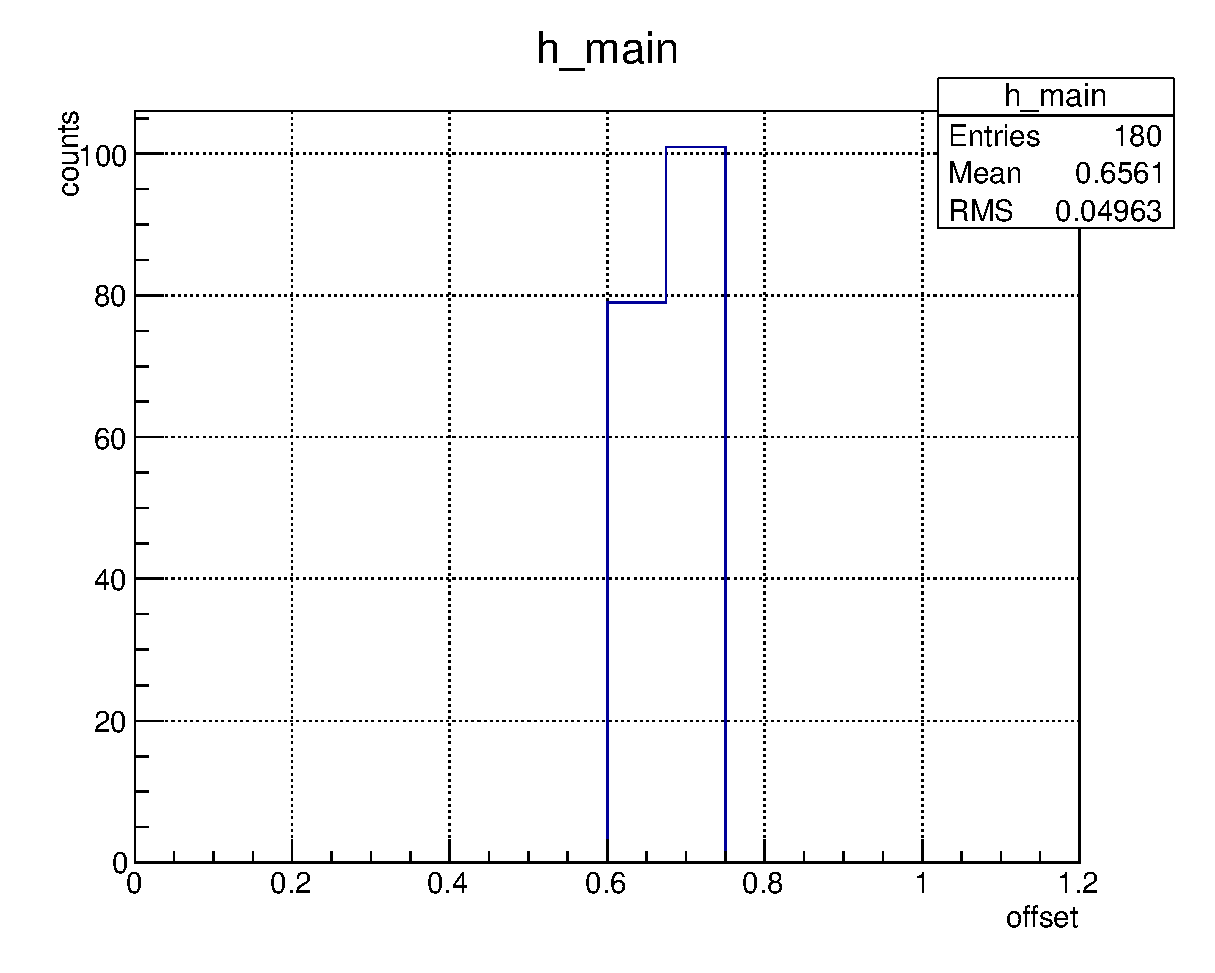
\includegraphics[width=0.8\textwidth]{chi_063_5k.eps}
	\centering
	\caption{ Bias estimation distribution for 5k data. 50k events for core template histograms. True bias is 0.063 mm. 1 bin = 0.1 mm. } 
	\label{fig:chi_063_5k}
	\end{figure}
	
	
	\section{Калібровочна крива}
	
	\subsection{Знаходження часу дрейфу}
	Після проходження зарядженої чатинки через об’єм дрейфової трубки вздовж треку виникають електрон іонні кластери, які під дією сильного електричного поля починають дрейфувати до відповідних електродів викликаючи струм у електричному колі дрейфової трубки. Слідом, ненульовий струм кола дрейфової трубки відповідає руху зарядів в о’бємі трубки. Час дрейфу найближчих до аноду електронів містить інформацію про положення треку в трубці, тож по моменту часу переднього фронту сигналу можна відновити положення треку, а точніше радіус кола дотичного до треку і паралельного трубці. Надалі будемо позначати {\it часом дрейфу} проміжок часу від моменту появи треку до перевищення вихідним сигналом певного порогового значення(зелена штрихована лінія на Рис. \ref{fig:signal_example}).
	
	\subsection{Джерела похибок}
	
	\begin{itemize}
		\item Природна складова похибки визвана розподілом кластерів іонізованих атомів вздовж треку MIP-частинки.\par
		\item Похибка пов’язана безпосереньо з дрейфом електронів та йонів в трубці. Залежить від параметрів електричного поля та складової газу в трубці.
		\item Похибка пов’язана з ефектами поширення заряду від електромагнітної лавини в дроті.
		\item Фактори електроніки -- функція відгуку електроніки.
	\end{itemize}
	
	\subsection{Геренерація шуму}
	Шум -- штука непердбачувана, і дуже залежить від технологічного процесу виготовлення складових елементів детекторної систреми. Шум в кінцевому результаті дуже впливає на якість вихідних даних детектора: його ефективність реєстрації, роздільну здатність.
	
	Шум зараз особливо важко оцінити, так як робочих екземплярів дрейфових трубок ще нема, і front-end електроніки в тому ж числі нема.
	
	Тож задамо шум з огляду детекторних установок подібного типу.
	
	Програмний пакет Garfield дозволяє задати значення струму шуму через імовірнісну функцію розподілу. Підберемо такий розподіл струму, щоб вихідна напруга перед дискримінатором (умовно кінцева напруга) була розподілена за гаусом 
	$P_{\mu,\sigma}(x) = Ae^{\frac{-(x-\mu)^2}{2\sigma^2}}$ 
	з середнім розподілу $\mu=0$ та з середнім квадратичним розподілом рівним сигналу від дрейфу 2000 електронів $ \sigma = 2000e$ -- так званий electric noise charge (ENC). Приклад сигналу шуму зображено на Pис. \ref{fig:signal_example}
	
	Дане питання одне із слабких місць даної симуляції і в майбутньому будуть проводитися зміни. Тож дана частина є нічим іншим як костиль.

	
	\section{Знаходження параметрів калібровочної кривої}
	
	Калібровочною кривою в даному випадку будемо називати функцію, яка є оптимально відповідність між часом дрейфу та нійблільш імовірним положенням треку(наприклад радіус кола, дотичного до лінії треку частинки концентричного до поперечного профілю трубки).\\
		
	\subsection{Випадок центрованого дроту}
	До початку розглянемо випадок, коли дріт трубки розташований строго по центру. Частинки, що проходять крізь дрейфову трубку на однаковій відстані мають викликати сигнал з однаковими часовими характеристиками зростаючого фронту (Рис. \ref{fig:track_reconstruction}). 
	
	Знаючи час дрейфу можемо відновити дотичне до треку коло. Якщо ж напрямок поширення частинки відомий то кількість можливих положень частинки зводиться до двох. На експерименті очікується, що дрейфові трубки будуть розташовані в площині перпендикулярній до напрямку пучка. Тож залишається серед двох дзеркальних треків вибрати один. Ця задача легко вирішується вже в процесі комбінаторики відновлення треку по хітах.
	
	\begin{figure}[h]
	\begin{tikzpicture}
	
	\tikzset{snake it/.style={decorate, decoration=snake}}
	
	\draw (0,0) circle (4);
	
	\draw[ultra thick] (0,0) circle (0.05);
	\node[below] at (0,0) {wire};
	
	\draw[thick,->] (0,0) -- (1.6,1.6);	
	\node at (1.5,0.7) {$r_{track}$};

	\draw[thick,->] (0,0) -- (-4,0);	
	\node[above right] at (-4,0) {$r_{tube}$};
		
	\draw[thick,->] (-6,2.3) -- (6,2.3);
	\node[above] at (-5,2.3) {$particle$};
	
	\draw[ultra thick, gray, dashed, ->] (-6,-2.3) -- (6,-2.3);
	
	\draw[ultra thick,gray,dashed] (0,0) circle (2.3);
	\node[below] at (3,-2.3) { $r_{reconstructed}$};
	
	\draw[thick,orange] (-3.0,2.3) circle(0.05);
	\draw[thick,orange] (-2.7,2.3) circle(0.05);
	\draw[thick,orange] (-2.6,2.3) circle(0.05);
	\draw[thick,orange] (-2.5,2.3) circle(0.05);
	\draw[thick,orange] (-2.1,2.3) circle(0.05);
	\draw[thick,orange] (-1.8,2.3) circle(0.05);
	\draw[thick,orange] (-1.0,2.3) circle(0.05);
	\draw[thick,orange] (-0.6,2.3) circle(0.05);
	\draw[thick,orange] (-0.5,2.3) circle(0.05);
	\draw[thick,orange] (0.26,2.3) circle(0.05);
	\draw[thick,orange] (0.4 ,2.3) circle(0.05);
	\draw[thick,orange] (1.3 ,2.3) circle(0.05);
	\draw[thick,orange] (1.56,2.3) circle(0.05);
	\draw[thick,orange] (1.96,2.3) circle(0.05);
	\draw[thick,orange] (2.22,2.3) circle(0.05);
	\draw[thick,orange] (2.48,2.3) circle(0.05);
	\draw[thick,orange] (2.68,2.3) circle(0.05);
	\draw[thick,orange] (2.88,2.3) circle(0.05);
	\draw[thick,orange] (3.00,2.3) circle(0.05);
	
	\draw[red,snake it](-0.6,2.3) -- (0,0);
	\draw[red,snake it](-0.5,2.3) -- (0,0);
	\draw[red,snake it](0.26,2.3) -- (0,0);
	\draw[red,snake it](0.4,2.3) -- (0,0);
	\node[] at (-0.3,1) {drift path};
	
	\end{tikzpicture} 
	\caption{Schematic view of a particle passing the straw and producing
ionization clusters. The ionization cluster electrons drift to the wire and
induce the signal. Only the earliest signal is detected. The closest distance
from the track to the wire, $r_{track}$, and radius of the straw, $r_{tube} = 2.45 mm$, are also indicated.}
	\label{fig:track_reconstruction}
	\end{figure}
	
	\begin{figure}[h]
	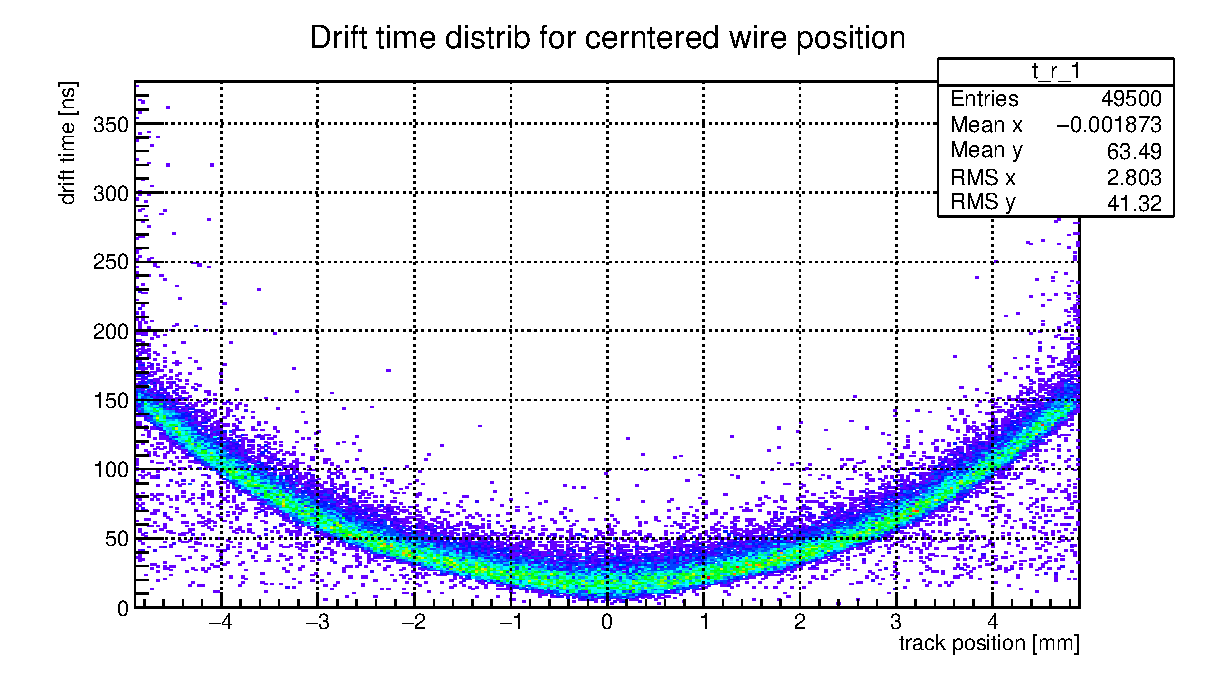
\includegraphics[width=0.8\textwidth]{t_r_distr_00.eps}
	\centering
	\caption{ Distribution of drift time $t_{drift}$ as function of track position $r_{track}$ relatively to the tube center} 
	\label{fig:t_r_distr_00}
	\end{figure}
	
	Калібровочну криву будемо знаходити з апроксимації розподілу $t_{drift}(r)$ Рис.\ref{fig:t_r_distr_00}.
	
	
	Instead of using the average value of the drift time residuals, a fit to the distribution
of unbiased drift time residuals is performed in a narrow range around
the peak. This allows to reduce the contribution of incorrectly assigned hits

	Для ясності опишемо дану процедуру поетапно
	\begin{enumerate}
	\item Оскільки TR розподіл симетричний Рис \ref{fig:t_r_distr_00}, то для підвищення статистики будемо аналізувати їх "суму".
	\item з TR розподілу рис.\ref{fig:t_r_distr_00} будуємо структурну діаграму шляхом розбиття даних на секції вздовж $r_{track}$ (ось Х) і знаходимо середнє для таких вибірок.
	\item як видно з рис.\ref{fig:t_r_distr_00} в симуляціях є досить багато шуму - точки поза головним "стержнем" розподілу. Тому для більш точних результатів в побудові RT залежності цього шуму слід позбавитися. Як варіант пропоную наступний критерій: вважати шумами всі точки, які знаходяться на відстані більше $2 \sigma $ від середнього вибірки для кожної із секцій від першої ітерації.
	\item для "відфільтрованих" даних повторюємо пункт №2;
	\item Апроксимуємо точки середнього з вибірок функцією (\ref{eq:fit_tr})
	\begin{equation}
		y = e^{a_0 +a_1x}
		\label{eq:fit_tr}
	\end{equation}
	\item Знаходимо RT відношення як оберенену до (\ref{eq:fit_tr})  функцію. Результат зображено червоною лінією на рис. \ref{fig:calibration_00}
	\end{enumerate}
	
	
	В даному випадку калібровочною кривою буде однозначна відповідність між часом дрейфу і радіусом дотичного кола.
	
	Для знаходження кривої $r(t)$ складемо дві гілки розподілу Рис. \ref{fig:t_r_distr_00} (праворуч і ліворуч нуля), 
	
	
	 інвертуємо розподіл $t_{drift}(r_{track}) \longrightarrow r_{track}(t_{drift})$ і виконаємо підгонку розподілу функцією виду (\ref{eq:calibration_func}).
	
	\begin{equation}
		\label{eq:calibration_func}
		r(t) = a_1 log(t) + a_2
	\end{equation}
	
	\begin{figure}[h]
	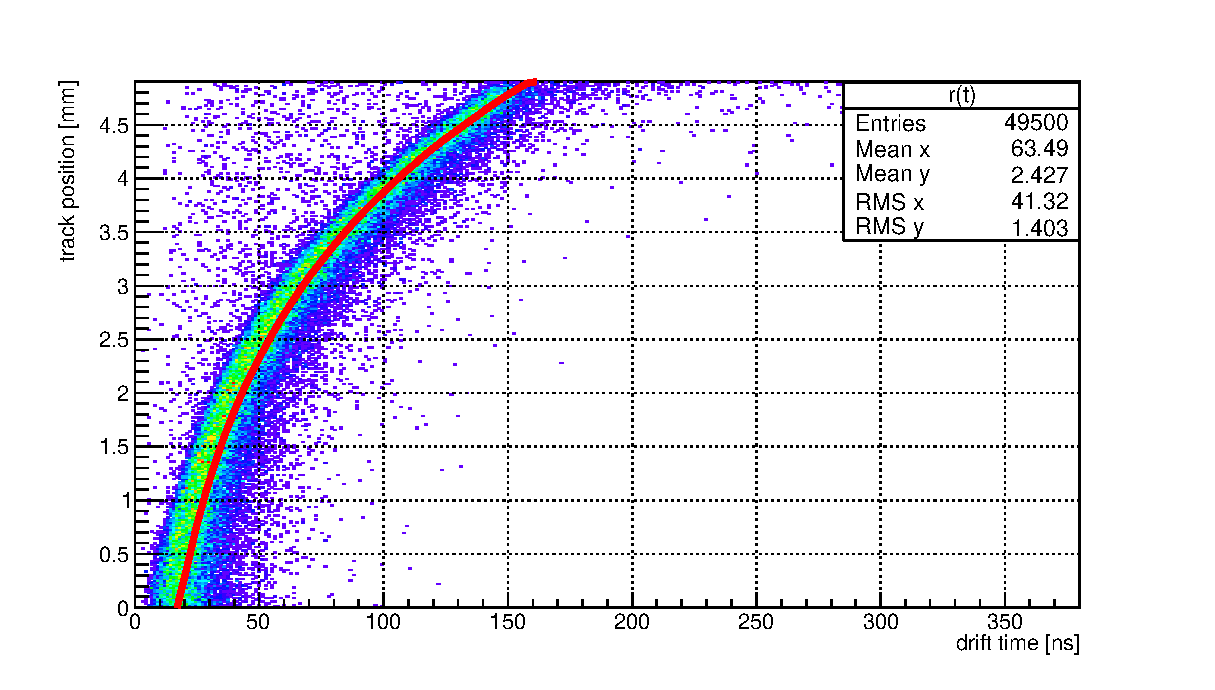
\includegraphics[width=0.7\textwidth]{rt_calibration.eps}
	\centering
	\caption{ RT-ralation(calibration line, figured in red color) between drift time $t_{drift}$ and distance from the  track $r_{track}$ .  The fit is performed in the range of
$0 < t_{drift} < 150 ns$ and $|r| < 4.9mm$ }
	\label{fig:calibration_00}
	\end{figure}
	
	Далі наводимо параметри калібровочної кривої як результат фітування розподілу $t_{drift}(r)$ Рис. \ref{fig:calibration_00} 
	
	\begin{itemize}
		\item $a_1 = 2.231 \pm 0.008$
		\item $a_2 = 0.448 \pm 0.002$
	\end{itemize}
	
	\subsubsection{Precision of track reconstruction}
	Похибкою вимірювання положення треку будемо називати різницю між дійсним положенням треку $r_{track}$ and reconstructed $r_{rec}$. Дану точку відобразим на графіку з відхиленням по осі Y та дійсним положенням треку по осі X. Для більшої наглядності ситуації з розподілом точок на графіку зобразимо цю ж інформацію у вагляді діаграми густини точок а також у виляді труктурної діаграми для  оцінки абсолютної похибки.
	
	Варто зазначити, калібровочна крива не проходить через точку $(0;0)$, то значення часу дрейфу ліворуч від кривої будемо співставляти центральний трек (такий, що проходить через центр дрейфової трубки $r=0$). Схоже правило застосовується для сигналів з часом дрейфу більшим за діапазон охоплений калібровочною кривою - таким сигналам $r_{reconstructed}$ присвоюється значення $r_{tube} = 4.9mm$.
	
	\begin{figure}[h]
	\centering
		\subfloat[Distribution of  $r_{track} - r_{rec}$ value]{
			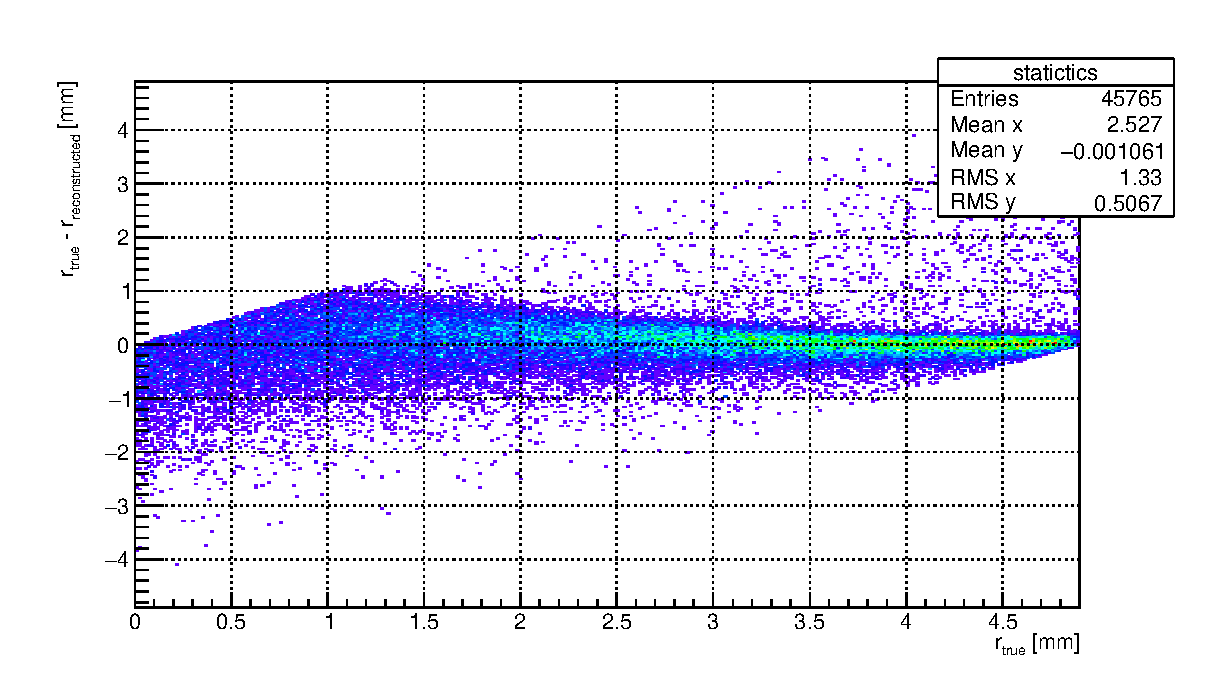
\includegraphics[width=0.45\textwidth]{difference_map_00.eps} 
			\label{fig:precision_00} }%
		\qquad
		\subfloat[projection of (a) along ]{
			\includegraphics[width=0.45\textwidth]{delta_structed.eps} 
			\label{fig:delta_sructed_00} }%
		\caption{Distribution of Розподіл різниці між дійсним і реконструйованим положенням треку в трубці $\bigtriangleup_{r_{track} - r_{rec}}$ від 49500 подій. Структурна діаграма розподілу точок у вападку строго центрального положення дроту дрейфової трубки}
	\end{figure}
	
	Як видно з простого аналізу діаграми Рис. \ref{fig:precision_00} \ref{fig:delta_sructed_00} точність реконструкції позиції треків лежить в діапазоні $(0.1 \dots 0.2) mm$. 
	
	\subsection{Випадок зміщеного дроту}
	Знаходження калібровочної кривої, якщо її так можна назвати, для випадку зміщеного дроту дещо відрізняється від описаного вище центрального випадку. Це пов’язано з несиметричністю розподілу ``час дрейфу - положення треку'' Рис. \ref{fig:tr_distr_15}. Тож необхідно знайте не одну, а дві калібровочні криві, причому необхідно розділення даних(на гілки більшу-меншу) що неможливо без попередньої оціки величини зміщення дроту від центрального положення.
	
	\begin{figure}
		\centering
		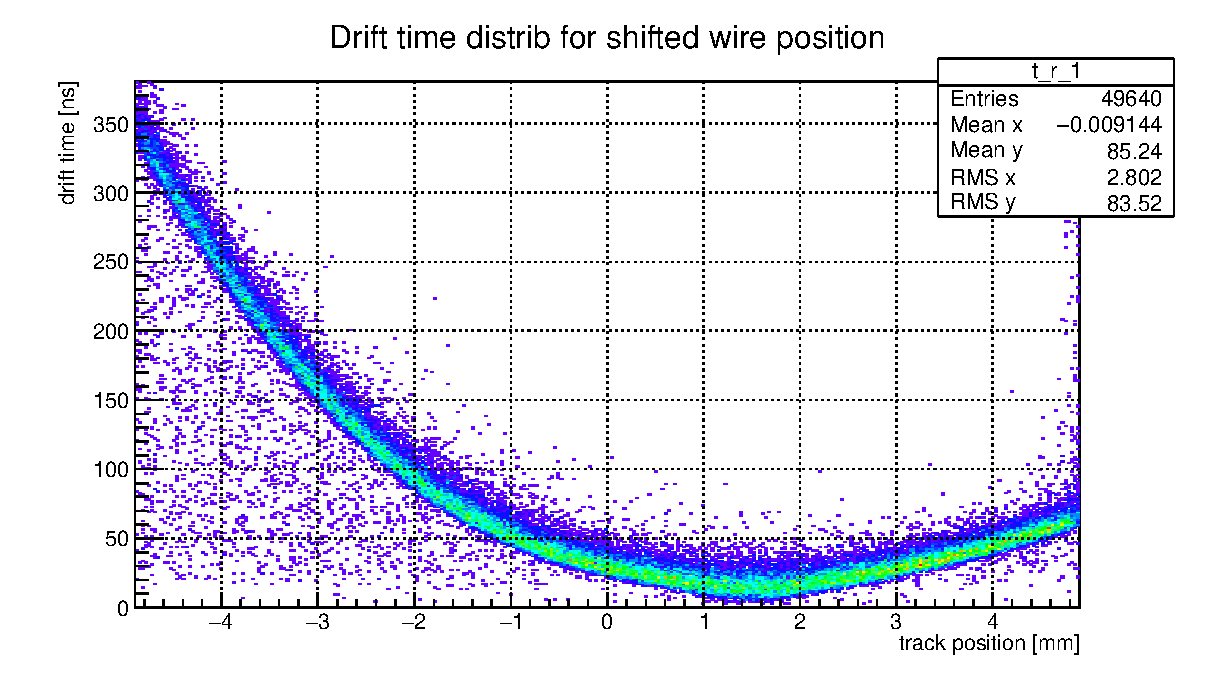
\includegraphics[width = \textwidth]{tr_distr_15.eps}
		\caption{TR-distribution for 1.5 mm shifted wire}
		\label{fig:tr_distr_15}
	\end{figure}
	
	Як видно з Рис \ref{fig:tr_distr_15} фігура розподілу змінилася не значно, а лише зсунулася на стале значення, рівне зміщенню дроту.
	
	Використаємо цю хитрість для розбиття даних на дві частини - дві гілки в RT розподілі. Від так ми можемо для  кожної гілки знайти свою власну калібровочну криву.
	
	
	\subsection{ Випадок максимального провисання дроту}
	Як видно з розрахунку профілю провисання, максимальне значення відхилення дроту від центру трубки становить $1.49~mm$. В цьому випадку очікуємо великих статистичних похибок. Густина точок розподілу та структурна діаграма для даного розподілу точок зображена на рисунку.
	
	\begin{figure}[h!]
%	\includegraphics[width=0.8\textwidth]{densityMap1_5mmSag.eps}
	\centering
	\caption{ Діаграма густини розподілу точок у вападку зміщення дроту дрейфової трубки на $1.5 mm$ від центрального положення}
	\end{figure}
	
	З графіків видно, що систематична похибка локалізації треків, пов’язана зі зміщенням дроту від центрального положення.
	В результаті поле всередині трубки міняється і задача стає несиметричною відносно центру трубки.
	
	\subsection{ Порівняння розподілів для центрального та зміщеного позицій дроту в трубці}	
	Наведемо порівнняння гістограм для центрального та зміщеного позицій дроту для вибірки треків в околі дроту та на відстані 2 мм від нього.
	
	\begin{figure}[h!]
	\includegraphics[width=0.8\textwidth]{bin0_0mm.eps}
	\centering
	\caption{ Порівняння розподілу реконструкції позицій треків для центрального положення дроту та вападку зміщення дроту дрейфової трубки на $1.5 mm$ від центрального положення для треків які проходять близько до центру трубки}
	\end{figure}
	
	\begin{figure}[h!]
	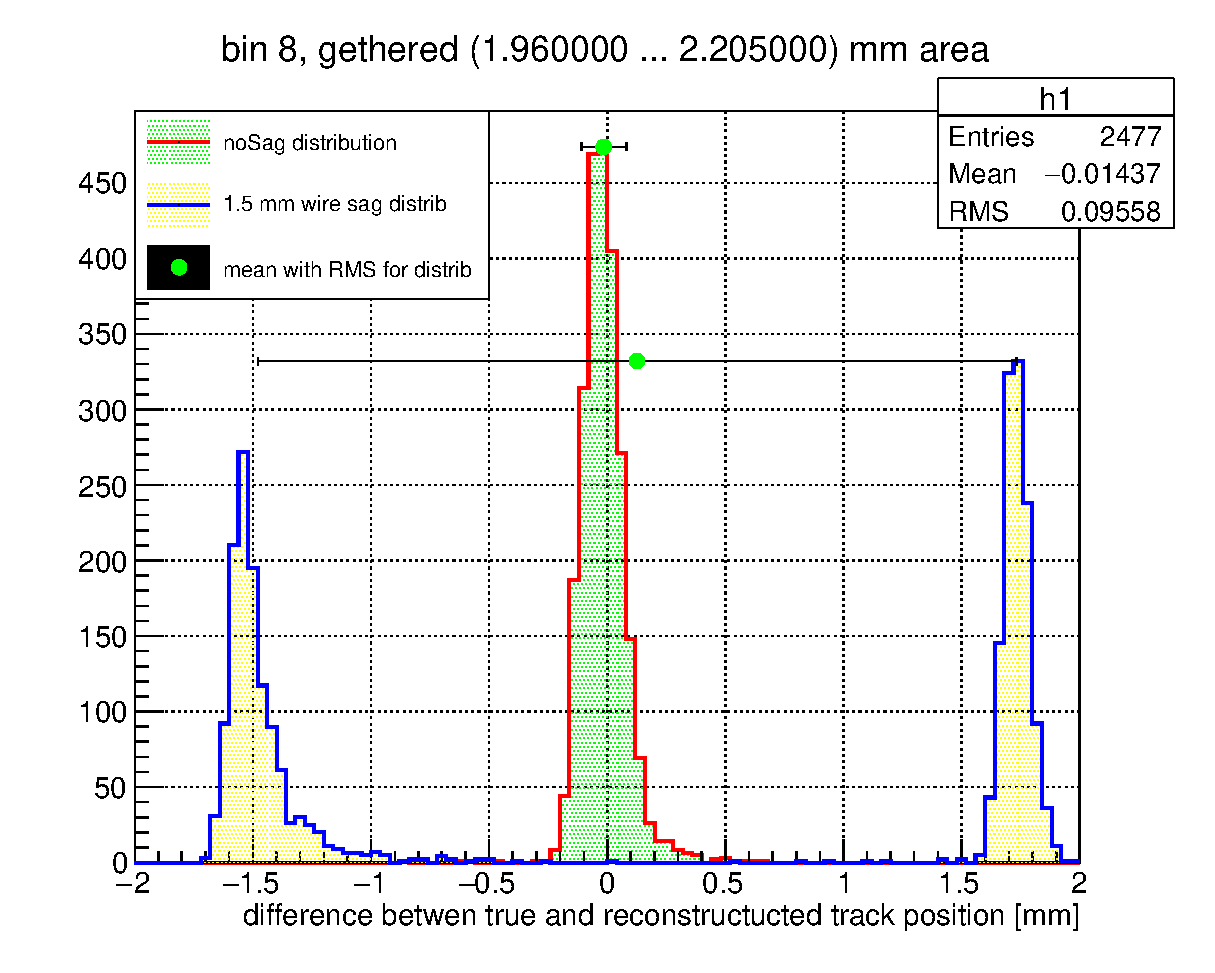
\includegraphics[width=0.8\textwidth]{bin8_2mm.eps}
	\centering
	\caption{ Порівняння розподілу реконструкції позицій треків для центрального положення дроту та вападку зміщення дроту дрейфової трубки на $1.5 mm$ від центрального положення для треків які проходять дотично до кола радусом $2mm$  коцентричного з трубкою}
	\end{figure}
	
	Цілком логічно припускати, що електроніка реєструватиме час дрейфу відмінний від триманого нами від симуляцій описаних вище. Тож необхідним буде врахувати внесок від електроніки. Ситуація ускладнюється тим що окрім форми вхідного сигналу потрібно знати ще й амплітуду сигналу(сумарний заряд зібраний з треку з урахуванням підсилення).
	
\newpage
\begin{thebibliography}{00}
	\bibitem{garfield} http://garfield.web.cern.ch/garfield

	\bibitem{kozlinskiy}  thesis Kozlinskiy.pdf 
	
\end{thebibliography}
	
\end{document}